% fig_method.tex -- Figure 1: the method in pictures (TikZ, drawn by hand; absolute coordinates in cm, natural width 17.6 cm = \textwidth).
%   (a) test time: one forward pass of the frozen denoiser, stopped at block X; two descriptors: f (mean and std of the upright block U)
%       and z (one number per block up to X: the comb under the blocks).
%   (b) once, before: the train images in the eight orientations of the square: the upright bank u and the bank o of the seven others.
%   (c) per descriptor: the distance to the R-th nearest entry of u and to the 7R-th nearest entry of o (drawn for R = 1: the nearest
%       navy dot lies on the solid circle, the seventh nearest grey square on the dashed circle).
%   Colours: black, navy (upright side: U, f, bank u), red (X, z, the input in panel c), grey (the re-oriented bank).  Schematic.
\providecommand{\figlab}{\fontsize{6.2}{7.6}\selectfont}
\begin{tikzpicture}[font=\figlab, >={Stealth[length=1.6mm, width=1.3mm]}, line join=round, line cap=round,
  lab/.style={font=\figlab, inner sep=1pt, align=center}, ttl/.style={font=\scriptsize, anchor=south west, inner sep=0pt}]
%% ================================================================ (a) test time
\node[ttl] at (0,0.15) {\textbf{(a)}\ テスト時：1回の順伝播を途中で打ち切り, 2つの記述子を読む};
\node[inner sep=0, draw=black, line width=0.6pt] (img) at (0.6,-1.55) {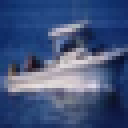
\includegraphics[width=1.05cm]{figs/o0.png}};
\node[lab, anchor=north] at (0.6,-2.16) {入力画像 $x$};
\draw[->] (1.2,-1.55) -- node[above, lab] {$+\sigma_1\varepsilon$} (1.87,-1.55);
% the blocks of the denoiser, left edge / height: encoder (32, 32, 16, 16, 8, 8), decoder (8, U at 8, 16, X at 16), then two blocks at 32
% that are not computed.  One red tick per block up to X: one number per block (the amplitude), collected on the red line.
\def\ybus{-2.68}
\foreach \xl/\h in {1.95/1.8, 2.22/1.8, 2.57/1.25, 2.84/1.25, 3.19/0.78, 3.46/0.78, 3.81/0.78, 4.08/0.78, 4.43/1.25, 4.70/1.25}{
  \draw[redc, line width=0.5pt] ({\xl+0.1},{-1.55-\h/2}) -- ({\xl+0.1},\ybus);
  \fill[redc] ({\xl+0.1},\ybus) circle (0.035);}
\foreach \xl/\h in {1.95/1.8, 2.22/1.8, 2.57/1.25, 2.84/1.25, 3.19/0.78, 3.46/0.78, 3.81/0.78, 4.43/1.25}
  \draw[black, fill=white, line width=0.7pt] (\xl,{-1.55-\h/2}) rectangle ++(0.2,\h);
\draw[navyc, fill=navyc!35, line width=0.9pt] (4.08,-1.94) rectangle ++(0.2,0.78);
\draw[redc, fill=redc!25, line width=0.9pt] (4.70,-2.175) rectangle ++(0.2,1.25);
\foreach \xl in {5.05, 5.32}
  \draw[black!45, densely dashed, line width=0.5pt] (\xl,-2.45) rectangle ++(0.2,1.8);
\draw[redc, line width=0.5pt] (2.05,\ybus) -- (4.80,\ybus);
\node[lab, anchor=south] at (2.8,-0.6) {エンコーダ};
\node[lab, anchor=south west] at (4.34,-0.6) {デコーダ};
\node[lab, anchor=south east, text=navyc] at (4.15,-1.15) {\textbf{U}};
\node[lab, anchor=south, text=redc] at (4.80,-0.92) {\textbf{X}};
\node[lab, anchor=north west, text=black!60] at (4.98,-2.5) {計算しない};
\node[lab, anchor=north west, align=left] at (0.0,-2.98) {凍結したノイズ除去器\\\textcolor{navyc}{\textbf{U}}：正立ブロック\\\textcolor{redc}{\textbf{X}}：打ち切りブロック};
% the two descriptors
\node[draw=navyc, rounded corners=2pt, line width=0.8pt, inner sep=3pt, align=left, font=\figlab, text width=21mm, anchor=north west] (fbox) at (6.1,-0.45)
  {$f$：U の出力の,\\チャネルごとの\\平均と標準偏差};
\node[draw=redc, rounded corners=2pt, line width=0.8pt, inner sep=3pt, align=left, font=\figlab, text width=21mm, anchor=north west] (zbox) at (6.1,-2.92)
  {$z$：X までの\\各ブロックの出力から\\数値を1つずつ};
\draw[->, navyc, line width=0.7pt] (4.18,-1.16) -- (4.18,-0.12) -- (7.2,-0.12) -- (7.2,-0.45);
\draw[->, redc, line width=0.7pt] (3.425,\ybus) -- (3.425,-3.43) -- (6.1,-3.43);
%% ================================================================ (b) the banks
\node[ttl] at (8.75,0.15) {\textbf{(b)}\ 事前：8通りの向き};
\draw[black!45, rounded corners=3pt] (8.75,-0.15) rectangle (12.25,-4.38);
\foreach \k/\xc/\yc in {1/10.11/-0.74, 2/10.89/-0.74, 3/11.67/-0.74, 4/9.33/-1.52, 5/10.11/-1.52, 6/10.89/-1.52, 7/11.67/-1.52}
  \node[inner sep=0, draw=black!55, line width=0.5pt] at (\xc,\yc) {\includegraphics[width=0.7cm]{figs/o\k.png}};
\node[inner sep=0, draw=navyc, line width=1.5pt] at (9.33,-0.74) {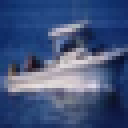
\includegraphics[width=0.7cm]{figs/o0.png}};
\draw[navyc, line width=1.0pt] (8.98,-2.31) rectangle ++(0.15,0.15);
\node[lab, anchor=west, align=left, text=navyc] at (9.2,-2.37) {そのまま(正立)の $N$ 枚\\→ バンク $u$};
\draw[black!55, line width=0.6pt] (8.98,-3.08) rectangle ++(0.15,0.15);
\node[lab, anchor=west, align=left, text=black!75] at (9.2,-3.14) {向きを変えた $7N$ 枚\\→ バンク $o$};
\node[lab, anchor=west, text=black!60] at (8.95,-3.95) {ノイズ $\varepsilon$ は変換しない};
%% ================================================================ (c) the score
\node[ttl] at (12.55,0.15) {\textbf{(c)}\ 2つのバンクへの近さを読む};
\draw[black!45, rounded corners=3pt] (12.55,-0.15) rectangle (17.6,-4.38);
% the two banks, the two circles and the input: written by gen/mk_schem.py in the coordinates of the panel
\begin{scope}[shift={(12.55,-0.15)}]
% written by gen/mk_schem.py: the two banks of Figure 1 (c), drawn for R = 1 (6 navy dots = u, 42 grey squares = o)
\foreach \p in {(1.612,-1.083),(1.380,-1.980),(1.120,-0.480),(0.780,-1.220),(0.380,-0.620),(0.360,-1.820)} \fill[navyc] \p circle (0.055);
\foreach \p in {(3.027,-1.223),(3.091,-1.535),(3.077,-0.925),(3.112,-1.790),(2.997,-0.662),(3.236,-1.128),(3.056,-2.008),(3.240,-2.415),(3.259,-2.064),(3.496,-2.116),(3.523,-0.975),(3.537,-0.342),(3.541,-1.408),(3.551,-1.697),(3.564,-2.415),(3.796,-2.094),(3.827,-0.968),(3.833,-1.304),(3.866,-0.601),(3.866,-0.255),(3.885,-1.756),(3.896,-2.420),(4.161,-0.666),(4.170,-1.307),(4.175,-0.324),(4.181,-2.452),(4.182,-1.657),(4.203,-2.001),(4.431,-2.376),(4.454,-1.760),(4.506,-1.039),(4.520,-1.347),(4.522,-2.001),(4.523,-0.244),(4.529,-0.644),(4.775,-0.620),(4.789,-0.342),(4.801,-2.352),(4.814,-1.411),(4.826,-1.728),(4.845,-1.059),(4.846,-2.002)} \fill[black!45] \p ++(-0.04,-0.04) rectangle ++(0.08,0.08);
\draw[navyc, line width=0.6pt] (2.150,-1.300) circle (0.580);
\draw[black!60, densely dashed, line width=0.6pt] (2.150,-1.300) circle (1.150);
\draw[navyc, line width=0.6pt] (2.150,-1.300) -- node[pos=0.62, above right, inner sep=1pt, text=navyc, font=\figlab] {$r^{u}_{R}$} (1.612,-1.083);
\draw[black!65, line width=0.6pt] (2.150,-1.300) -- node[pos=0.80, below left, inner sep=0.5pt, text=black!75, font=\figlab] {$r^{o}_{R}$} (3.056,-2.008);
\node[star, star points=5, star point ratio=2.2, fill=redc, inner sep=1.2pt] at (2.150,-1.300) {};

\end{scope}
\fill[navyc] (12.8,-2.80) circle (0.055); \node[lab, anchor=west, text=navyc] at (12.9,-2.80) {正立の train 画像($u$)};
\node[star, star points=5, star point ratio=2.2, fill=redc, inner sep=0.95pt] at (15.85,-2.80) {}; \node[lab, anchor=west] at (15.97,-2.80) {入力};
\fill[black!45] (12.75,-3.12) rectangle ++(0.1,0.1); \node[lab, anchor=west, text=black!75] at (12.9,-3.07) {向きを変えた train 画像($o$)};
\node[draw=black, rounded corners=2pt, line width=0.9pt, inner sep=3pt, align=left, font=\figlab, text width=45mm, anchor=north] at (15.075,-3.27)
  {密度：$r^{u}_{R}$ が小さいほど高い\\比：$r^{o}_{R}/r^{u}_{R}$ が大きいほど高い\\$s(x)=J_f(x)+J_z(x)$\ \ [式~(\ref{eq:J}),\,(\ref{eq:score})]};
\end{tikzpicture}
